\documentclass[12pt, a4paper]{article}

% Ru lang stuff
\usepackage [utf8x] {inputenc}
\usepackage [T2A] {fontenc}

% running titles 
\usepackage{fancybox}
\usepackage{fancyhdr}

% for last page number
\usepackage{lastpage}

%for colored tablets cells
\usepackage{colortbl}

% for Ru text in formulas
\usepackage[warn]{mathtext}

% for captions 
\usepackage[labelsep=period]{caption}
\usepackage{capt-of}

% for colored hyperrefs
\usepackage{xcolor}
\usepackage{hyperref}

% for pictures 
\usepackage{graphicx}

% for coll math
\usepackage{amsmath}
\usepackage{amsthm}

% path to all pictures
\graphicspath{{picks/}}

% for enumerates
\usepackage[shortlabels]{enumitem}

% for diff running titles on pages with diff parity
\usepackage{ifthen}
\usepackage{pdfpages}
\usepackage[strict]{changepage}

%for drawings
\usepackage{tikz}
\usetikzlibrary{calc}
\usetikzlibrary{decorations.pathmorphing}

% for good text in tablets
\usepackage{array}

% upgrading tables
\newcolumntype{P}[1]{>{\centering\arraybackslash}p{#1}}
\newcolumntype{M}[1]{>{\centering\arraybackslash}m{#1}}


% dock fields 20 15 15 35
\usepackage[left=12mm, top=12mm, right=15mm, bottom=28mm, nohead, footskip=10mm]{geometry}

% for cool tables
\usepackage{multirow}

% for different section/subsection/subsubsection styles in contents and doc
\usepackage[english, russian]{babel}

\usepackage{amsmath}

% for cool tables
\usepackage{tabularx}

\usepackage{fancyhdr,color}
\usepackage{amssymb}
% page style setup (for running titles)
\pagestyle{myheadings}
\pagestyle{fancy}
\fancyhead[C]{}
\fancyhead[R]{\rightmark}
\fancyfoot[L]{ОВАиТК, ФПМИ, МФТИ}
\fancyfoot[C]{\textcopyright Павлов М.А.}
\fancyfoot[R]{\thepage}

\fancypagestyle{plain}{ %
    \fancyhf{} % remove everything

    % lines parameters
    \renewcommand{\headrulewidth}{0pt}
    \renewcommand{\footrulewidth}{0pt}



% running titles contents
    \lfoot{\textcolor{black!50}{Павлов М. А.,}}
    \rfoot{\textcolor{black!50}{\thepage}}
}

\newcommand{\sectionmark}[1]{\markboth
{\uppercase{\thesection\hspace{1em}#1}}% левая пометка
{\uppercase{\thesection\hspace{1em}#1}}% правая пометка
}% конец макроопределения

\theoremstyle{definition}
\newtheorem{ex}{Пример}[section]
\newtheorem{st}[ex]{Утверждение}

\title{Homework 4}
\author{Mikhail Pavlov \thanks{MIPT}}
\date{March, 2022}
\begin{document}

    \section{Домашнее задание за 4-ую неделю}

    \section*{Задание 1}

        Поскольку $N$ -- нормальная подгруппа, то в ней определена та же операция, что и в $G$.

        В таком случае $ab \in N, abab \in N \dots ababab\dots(m times)ab \in N$. Осталось доказать, что $(ab)^m = a^mb^m$.
        Докажем, что $abab = a^2 b^2$ с помощью ММИ:

        Из определения нормальной подгруппы $a^{-1} \cdot ab = ab \cdot a^{-1} \Rightarrow b = aba^{-1}$

        Отсюда получаем $abab = aaba^{-1}ab = aabb = a^{2} b^2$. Значит, $N$ содержит $a^2 b^2$

        Пусть верно для $k$. Докажем для $k + 1$: $ab \cdot (ab)^k = (ab)^k \cdot ab$

        $ab a^k b^k = a aba^{-1} a^k b^k = a^2 b a^{k-1} b^k = \dots = a^{k+1}b^{k+1} = \dots = a^k b^k \cdot ab$.

        Значит, $a^{k+1} b^{k+1} \in N$

    (*) Пользуемся свойством (доказано выше), что $b = a^{-1}ba$, подставляя вместо всех $b$ это значение, и доказываем,
    что достигается равенство, откуда следует, что $N$ содержит и то, и другое для любого целого $m$.

    \section*{Задание 2!}

    1. Берем группу $S_3$ и ее подгруппу $H = {e, (1,2)}$

    $H (1,3) = {(1,3), (1, 3, 2)}$, но $(1,3) H = {(1, 3), (1, 2, 3)} \Rightarrow$ подгруппа не является нормальной.

    \section*{Задание 3}

    Построим гомоморфизм $\phi: Z^3 \rightarrow Z : (x, y, z) \in Z^3 \rightarrow x + y + z \in Z$

    Т.к. $\phi$ -- сюръективно, то $Im f = Z$

    Т.к. $\phi$ -- гомоморфизм, то $Z^3/Ker \phi \cong Z$ -- это и будет искомой факторгруппой

    \section*{Задание 4}

    $(10a + 3b) - (8a + 9b) = 0 = 2a - 6b$

    Тогда имеем из (1): $5(2a) + 3b = 5(6b) + 3b = 33b = 0$ -- значит, группа конечная.

    $33b = 0 \Rightarrow 34b = b$, то есть $b = 34b = 4b + 30b = 4b + 10a = b$. То есть мы не можем выразить $a$ через $b$ (и наоборот).
    Значит, группа циклической не является.

    \section*{Задание 5}

        \begin{center}
            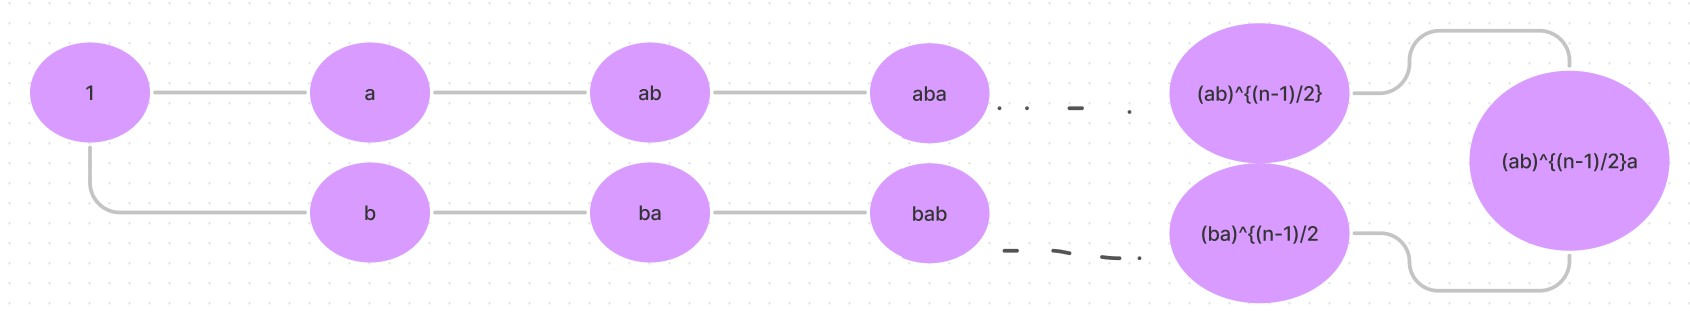
\includegraphics[scale=0.5]{picture1}
        \end{center}

    \textbf{Комментарий:} Здесь приведен случай для нечетного $n$. Если $n$ будет четным, то изображение графа будет таким же,
    но крайней правой вершиной будет $(ab)^{\frac{n}{2}}$. В процессе решения использовалось: $b = (ab)^{n-1}a$.

    \section{Домашнее задание за 4-ую неделю}

    \section*{Задача 6}

    \subsection{}
        $\phi : Q \rightarrow Q : {\forall x \in Q \rightarrow \phi(x) = \frac{1}{2}\{x\}}$

    \subsection{}
        Факт, что группа бесконечна, очевиден и следует непосредственно из теоремы о Гомоморфизме (то есть мы имеем факторгруппу по ядру,
        которая изоморфна гомоморфному образу группы, который в свою очередь бесконечен).

        Факт, что каждый элемент группы имеет конечный порядок, следует из счетности рациональных чисел.
\end{document}
